\documentclass{beamer}
\usetheme{Pittsburgh}
\beamertemplatenavigationsymbolsempty


\usepackage{amsmath}
\usepackage{amssymb}
\usepackage{bm} % For bold math symbols
\usepackage{graphicx}
\usepackage{tikz}



\usepackage{subfig} % Changed from subfigure (deprecated)
\usepackage{multirow}
\usepackage{multicol}
\usepackage{color}
\usepackage{url}
\usepackage{hyperref}
\usepackage{listings}
\usepackage[noend]{algorithm}
\usepackage{physics} 

\usepackage{animate}

% add image path
\graphicspath{{Images/}}






\DeclareMathOperator{\argmin}{argmin}
\DeclareMathOperator{\argmax}{argmax}






\title{Weekly Updates\\
\tiny{Wednesday, 26/03/2025}}
\author{Andrea Bonifacio}
\date{}

\begin{document}

\begin{frame}
\titlepage
\end{frame}


\begin{frame}{Where are we stuck?}
    \begin{itemize}
        \item I have a working code, but something's missing.
        \item In the paper, and in their code, they minimize some energy computed by a function which is not present in the code.
        \item By minimizing only the internal energy, the network have no information about the external forces.
        \item They used Saint-Venant Kirchhoff material model, while I used Neo-Hookean. But I don't think this is the issue.
    \end{itemize}
\end{frame}


\begin{frame}
    \frametitle{Example of the issue}
    \begin{itemize}
        \item Same visualization of last week.
        \item The network has learned to minimize the internal energy, but has no control on the linear modes output, which dominates the simulation.
        \item Objective function used:
        \[
              z_{n+1} = \underset{z}{\argmin}  \frac{1}{2h^2} \norm{n(z) - 2u_n + u_{n-1}}^2_M + E(n(z))
        \]
    \end{itemize}
\end{frame}

\begin{frame}
    \frametitle{Adding a term to the objective}
    \begin{center}
        \animategraphics[width=0.8\textwidth, autoplay, loop]{12}{Images/beam_linear/frames/frame}{0}{27}
    \end{center}
\end{frame}

\begin{frame}
    \frametitle{Dynamic simulation - Twisting Beam}
    \begin{itemize}
        \item This thing I made last week has no theoretical basis, but gave me an intuition that something was missing from my training.
        \item This simulation doesn't work better, but at least doesn't explode.
        \item I think that the external force is an information that the objective function should have.
        \[
            \begin{split}
                z_{n+1} = \underset{z}{\argmin}  \frac{1}{2h^2} \norm{n(z) - 2u_n + u_{n-1}}^2_M + E(n(z)) \\ + \text{some term that depends on the external force}
            \end{split}
        \]
    \end{itemize}
\end{frame}

\begin{frame}
    \frametitle{Animated Beam Deformation}
    \begin{center}
        \animategraphics[width=0.8\textwidth, autoplay, loop]{12}{Images/beam_deformation/frames/frame}{0}{43}
    \end{center}
\end{frame}


\begin{frame}
    \frametitle{Network Architecture}
    \begin{itemize}
        \item The network is a feedforward neural network.
        \item The input is the modal coordinate \( z \in \mathbb{R}^m \).
        \item The output is a correction on the displacement field \( \mathbf{y} \in \mathbb{R}^n \).
    \end{itemize}



\begin{center}
        
        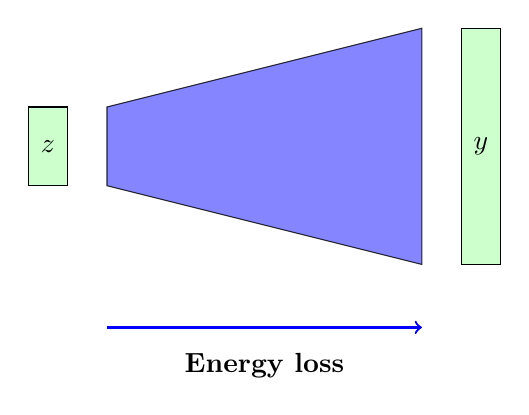
\begin{tikzpicture}
            % Modal coordinate (z)
            \draw[fill=green!20] (-3, 1) rectangle (-2.5,2);
            \node at (-2.75, 1.5) {$z$}; % Label inside the rectangle
            
            % Displacement (u)
            \draw[fill=green!20] (2.5,0) rectangle (3,3);
            \node at (2.75, 1.5) {$y$}; % Label inside the rectangle
            
            % Energy loss transition
            \draw[fill=blue!60,opacity=0.8] (-2,1) -- (2,-0) -- (2,3) -- (-2,2) -- cycle;
            \node[below] at (0,-1) {\textbf{Energy loss}};
            
            % Energy loss arrow
            \draw[thick,blue,->] (-2,-0.8) -- (2,-0.8);
        
        \end{tikzpicture}
\end{center}
    
\end{frame}





\begin{frame}
    \frametitle{My side quest}
    \begin{itemize}
        \item I was thinking about how to let the network be aware of the external forces during training.
        \item I need something like a map 
        \begin{align*}
            \mathbb{R}^m &\to \mathbb{R}^n \\
            z &\mapsto \text{external force}
        \end{align*}
        \item The idea is to obtain from the latent space \( z \), which describes a deformation, the external force that causes that deformation.
        \item I have no idea if such a map exists.
    \end{itemize}
\end{frame}

\begin{frame}
    \frametitle{My side quest}
        \begin{itemize}
            \item My idea was to use a neural network to approximate this map $\Phi: \mathbb{R}^m \rightarrow \mathbb{R}^n$, where $\Phi(z) = \hat{\mathbf{f}}$.
            \item I would construct a dataset $\mathcal{D} = \{(z_i, \mathbf{u}_i, \mathbf{f}_i)\}_{i=1}^N$ of deformations and corresponding external forces.
            \item The training loop would then be:
            \begin{enumerate}
                \item Predict $\hat{\mathbf{f}} = \Phi(z)$ from the latent vector $z$.
                \item Compute displacement field $\hat{u}$ using $\hat{\mathbf{f}}$ with a physics solver $\mathcal{S}(\hat{\mathbf{f}})$.
                \item Minimize the composite loss function:
                    $\mathcal{L} = \alpha\|\hat{u} - \mathcal{S}(\mathbf{f})\|_2^2 + \beta\|\hat{\mathbf{f}} - \mathbf{f}\|_2^2$
                \item Backpropagate the loss through the network-
                \item Repeat.
            \end{enumerate}
        \end{itemize}
\end{frame}

\begin{frame}
    \frametitle{My side quest}
    \textbf{The problem:}
    \begin{itemize}
        \item Using FEniCS is outrageously slow.
        \item I built a surrogate solver that uses LBGFS instead of Newton's method.
        \item I have problem with what I should minimize. 
    \end{itemize}
\end{frame}

\begin{frame}
    \frametitle{Challenges \& Next Steps}
        \begin{itemize}
            \item I am open to suggestions on how to proceed, I don't really have an idea.
            \item I tried building this side network in the last few days, but I keep failing to make it work.
            \item I think that to learn proper nonlinear modes we need information about the external forces.
            \item I am not sure if the map $\Phi$ exists, or if it is learnable.
        \end{itemize}
\end{frame}

% Q&A
\begin{frame}
    \begin{center}
        \color{blue} \Huge{Questions?}
    \end{center}

\end{frame}
\end{document}

